\documentclass[times, utf8, zavrsni, numeric]{fer}

\usepackage{booktabs}
\usepackage{graphicx}
\usepackage{caption}
\usepackage{subcaption}
\usepackage{svg}
\graphicspath{{./images/}}

\usepackage{listings}
\usepackage{color}

\definecolor{dkgreen}{rgb}{0,0.6,0}
\definecolor{gray}{rgb}{0.5,0.5,0.5}
\definecolor{mauve}{rgb}{0.58,0,0.82}

\lstset{frame=tb,
  language=Java,
  aboveskip=3mm,
  belowskip=3mm,
  showstringspaces=false,
  columns=flexible,
  basicstyle={\small\ttfamily},
  numbers=none,
  numberstyle=\tiny\color{gray},
  keywordstyle=\color{blue},
  commentstyle=\color{dkgreen},
  stringstyle=\color{mauve},
  breaklines=true,
  breakatwhitespace=true,
  tabsize=3
}

\lstnewenvironment{code}[1][]%
{\noindent\minipage{\linewidth}\medskip 
\lstset{basicstyle=\ttfamily\footnotesize,frame=single,#1}}
{\endminipage}

\begin{document}

% TODO: Navedite broj rada.
\thesisnumber{5672}

% TODO: Navedite naslov rada.
\title{Sustav za upravljanje i pretraživanje baze PDF dokumenata}

% TODO: Navedite vaše ime i prezime.
\author{Luka Čupić}

\maketitle

% Ispis stranice s napomenom o umetanju izvornika rada. Uklonite naredbu \izvornik ako želite izbaciti tu stranicu.
\izvornik

% Dodavanje zahvale ili prazne stranice. Ako ne želite dodati zahvalu, naredbu ostavite radi prazne stranice.
\zahvala{}

\tableofcontents

\listoffigures

\chapter{Uvod}
Korištenje računala za dohvat informacija (engl. \textit{information retrieval}) datira sve do četrdesetih godina dvadesetog stoljeća \cite{sanderson2012history}, daleko prije komercijalizacije računala, odnosno početka njihovog korištenja u osobne svrhe. Pogledaju li se samo neke od modernih primjena analize i pretraživanja teksta poput internetskih tražilica koje pretražuju ogromne količine podataka za zadani upit, osobnih asistenata na pametnim telefonima koji obrađuju izgovorene riječi pa sve do analize i prepoznavanja neželjenih elektroničkih poruka, očito je da je područje analize i pretraživanja teksta vrlo zastupljeno u današnjem digitalnom svijetu u kojem se količina informacija svake godine povećava eksponencijalno. Također je očito da je domena primjene  vrlo široka te da su analiza i pretraživanje teksta zastupljeni u praktički svakom području koje iziskuje nekakvu vrstu obrade, odnosno dohvata informacija iz teksta.

Tema ovog rada bit će obraditi neke od metoda za računalni prikaz dokumenata nad kojima će potom biti provedena usporedba sličnosti. Tako uspoređene dokumente bit će moguće prikazati grafički kako bi se dobio uvid u sličnost dokumenata. Teoretska podloga rada bit će popraćena programskom implementacijom koja će korisniku omogućiti upravljanje i pretraživanje lokalne baze PDF dokumenata te vizualizaciju iste.

U \ref{docmodel}. poglavlju opisan je prikaz, odnosno model prikaza dokumenata. Obrađeno je nekoliko metoda za rangiranje dokumenata, zajedno s matematičkom podlogom iza istih. Poglavlje \ref{chap:docsin2d} opisuje problematiku prikaza dokumenata u 2D-koordinatnom sustavu u svrhe vizualizacije sličnosti dokumenata te obrađuje korištene metode. U poglavlju \ref{chap:impl} opisana je implementacija programske potpore te su navedene korištene tehnologije i alati. Dan je pregled arhitekture programa te osnovnih funkcionalnosti. Naposlijetku, u \ref{chap:results}. poglavlju opisani su dobiveni rezultati te je dana njihova interpretacija.

Kroz ove 42 stranice bit će obrađena problematika modeliranja \cite{hitchhiker}, prikaza i usporedbe dokumenata u svrhe izračuna i vizualizacije njihovih međusobnih sličnosti.


\chapter{Model dokumenata}
\label{docmodel}

\section{Prikaz dokumenata}
\label{subchap:docmodel_docview}
Prije svega, valja definirati što u kontekstu analize i pretraživanja teksta predstavlja dokument. Dokument se neformalno može definirati kao kolekcija riječi. Ovakva kolekcija ne mora nužno biti skup, pošto dokument može imati više ponavljanja istih riječi, stoga se na dokument može gledati kao na poredanu kolekciju riječi u kojoj može biti ponavljanja  (ovakva kolekcija naziva se mnogoskup (engl. \textit{multiset}) o kojoj će više riječi biti u nastavku). Ovakva definicija dokumenta bit će bitna u nastavku za opis semantička sličnosti dokumenata \cite{Hausler2013}. Primjerice, neki dokument u kojemu se često pojavljuju riječi "računalo", "algoritam" te "memorija" očito će biti relevantan u kontekstu dokumenata vezanih za računarsku znanost. Postavlja se pitanje kako tako definirane dokumente prikazati u računalu. Jedan (smisleni) pokušaj bio bi predstaviti riječi kao vektore tako da svaka riječ dobije odgovarajući položaj u više-dimenzijskom prostoru. Ovakav model naziva se \textit{Word2Vec} te ima za posljedicu to da će semantički sličnije riječi biti bliže (odnosno da će pripadajući im vektori međusobno zatvarati manji kut) i obrnuto. Ovakav se model često koristi u kontekstu semantičke analize riječi, primjerice u pronalaženju sličnih riječi, sinonima, antonima itd. No ipak, u kontekstu ovog rada fokus će imati semantička sličnost \textit{dokumenata}. Stoga će za predstavljanje istih biti korišten tzv. model vreće riječi (engl. \textit{bag of words model}). U modelu vreće riječi, tekst dokumenta predstavljen je multiskupom riječi. Multiskup jest proširenje klasičnog skupa u smislu da dozvoljava više pojavljivanja elemenata, odnosno u ovom kontekstu, riječi. Kod modela vreće riječi, dakle, nije bitna semantika samih dokumenata, pa čak niti poredak riječi, već je bitno samo koje se riječi pojavljuju u određenom dokumentu, odnosno koja je učestalost njihovog pojavljivanja. Primjer modela vreće riječi prikazan je u nastavku:
Neka su zadani dokumenti $d_{1}$ = "Marko jako voli domaćice. Domaćice su ukusne." te $d_{2}$ = "Marko voli domaćice i programiranje." Za ovako zadane dokumente, prikazane su dobivene vreće riječi u JSON formatu:
\begin{align*}
BoW_{1} &= \text{\{"Marko":1, "jako":1, "voli":1, "domaćice":2, "su":1, "ukusne":1\}} \\
BoW_{2} &= \text{\{"Marko":1, "voli":1, "domaćice":1, "i":1, "programiranje":1\}}
\end{align*}

Iz dobivenih vreća riječi može se vidjeti koje se riječi nalaze u kojem dokumentu, odnosno koja je frekvencija njihovog pojavljivanja. \newline
Kako bi se uopće moglo započeti sa semantičkom analizom dokumenata, potrebno je imati kolekciju dokumenata (engl. \textit{dataset}; u daljnjem tekstu: zbirka) koji će se međusobno uspoređivati. Nakon što se osigura postojanje zbirke, korištenje modela vreće riječi zamišljeno je tako da se na početku iz svih dokumenata zbirke izvade sve riječi te potom uklone nebitne riječi (o kojima će više riječi biti u poglavlju \ref{chap:impl}) a od preostalih se riječi izgradi vektor koji će \textit{de-facto} predstavljati dokument. Ovako opisani model često je korišten u području obrade prirodnog jezika te dohvata informacija, kako iz dokumenata, tako iz drugih tekstovnih izvora.

U prethodnom primjeru prikazana je konstrukcija vreća riječi dvaju dokumenata. U tom primjeru, kao riječi koje se pojavljuju u vrećama uzete su sve riječi iz ulaznih dokumenata, što u praksi neće uvijek biti slučaj. Naime, u dokumentima se često znaju pronaći riječi koje nemaju nikakvo bitno značenje za sam dokument. Takve su riječi primjerice zamjenice, pomoćni glagoli, veznici itd. Ovakve riječi nazivaju se zaustavne riječi (engl. \textit{stop words}). To su riječi koje su učestale u nekom jeziku pa su nebitne za sam postupak analize teksta, jer ne doprinose sadržaju dokumenta \cite{allahyari2017}. Zaustavne se riječi stoga izbacuju iz vreća riječi te se zadržavaju samo riječi "bitne" za semantiku dokumenata — empirijski je pokazano da ovakvo uklanjanje zaustavnih riječi ima pozitivan utjecaj na daljnju obradu dokumenata. Primjeri nekih zaustavnih riječi u hrvatskom jeziku su: \textit{aha}, \textit{nešto}, \textit{okolo} te \textit{zaboga}.
Kako bi se dokumenti mogli predstaviti u obliku vreća riječi, potrebno je odrediti vokabular — skup riječi koje se nalaze u svim dokumentima promatrane zbirke. Poznavanje vokabulara ključno je za semantičku sličnost dokumenata, što će i biti pokazano kasnije. Iz dobivenog vokabulara potrebno je na početku obrade ukloniti zaustavne riječi iz već opisanih razloga. Osim zaustavnih riječi, dodatna obrada teksta može se obaviti tzv. stemanjem (engl. \textit{stemming}). Ova metoda ima zadaću svesti riječi na njihov kanonski oblik, kako bi riječi istog korijena bile svedene na istu riječ. Svođenje na kanonski oblik ne znači nužno i svođenje na morfološki korijen riječi. Primjerice, riječi "mačka", "mačkama" te "mačke" bile bi svedene na "mačk". Nebitno je dakle je li riječ napisana u jednini ili množini ili pak u kojem je padežu već je bitan samo njezin kanonski oblik.
Nakon stvaranja vokabulara te predobrade dokumenata (izbacivanje zaustavnih riječi, stemanje) sljedeći korak jest predstavljanje dokumenata. Radi praktičnosti, najčešća metoda predstavljanja dokumenata je uz pomoć vektora.
Najjednostavnija metoda vektorskog predstavljanja dokumenata jest binarna: za svaku riječ iz vokabulara naprosto se provjeri nalazi li se u danom dokumentu te ako se nalazi, odgovarajuća komponenta vektora (indeks riječi u vokabularu) bit će 1, a u suprotnom 0. Primjerice, za prethodno definirane dokumente $d_{1}$ i $d_{2}$, vokabular će nakon uklanjanja svih nebitnih znakova i stop riječi biti: V = \{"Marko", "jako", "voli", "domaćice", "ukusne", "programiranje"\}. Valja primijetiti kako su riječi "i" i "su" izbačene iz vokabulara. Koristeći binarnu metodu reprezentacije dokumenata, odgovarajući vektori će biti
\begin{align*}
{{d_{1}}=[1, 1, 1, 1, 1, 0]},
\end{align*}
\begin{align*}
{{d_{2}}=[1, 0, 1, 1, 0, 1]}
\end{align*}
zbog toga što prvi dokument ne sadrži riječ "programiranje" (zadnja komponenta) dok drugi dokument ne sadrži riječi "jako" (druga komponenta) te "ukusne" (predzadnja komponenta).
Nadograđujući se na prethodnu metodu, dolazi se do frekvencijskog prikaza vektora. Umjesto obične binarne reprezentacije u kojoj se pamti samo nalazi li se riječ u dokumentu ili ne, u frekvencijskom prikazu pamti se i koliko se puta određena riječ pojavljuje u dokumentu; komponente vektora zapravo su frekvencija (tj. broj) pojavljivanja određene riječi u dokumentu. Gledajući isti vokabular i dokumente kao u prethodnom primjeru, novi vektori će u ovom slučaju biti:
\begin{align*}
{{d_{1}}=[1, 1, 1, 2, 1, 0]}
\end{align*}
\begin{align*}
{{d_{2}}=[1, 0, 1, 1, 0, 1]}
\end{align*}
Jedina razlika u odnosu na prethodni primjer jest četvrta komponenta prvog vektora koja ukazuje na to da se riječ "domaćica" u prvom dokumentu pojavljuje dvaput.
Naposlijetku se dolazi i do najčešće metode vektorskog prikaza dokumenata u kontekstu analize i pretraživanja teksta — TF-IDF (engl. \textit{term frequency–inverse document frequency}) \cite{Stole2017}. Ova metoda zasniva se na dvije intuitivne pretpostavke:
\begin{itemize}
\item[$\bullet$] riječ je važnija za semantiku dokumenta što se češće u njemu pojavljuje (TF komponenta)
\item[$\bullet$] riječ je manje važna za semantiku dokumenta što se češće pojavljuje u drugim dokumentima (IDF komponenta).
\end{itemize}
TF i IDF dakle predstavljaju dvije komponente vektora kojima će se predstavljati dokumenti. Prva komponenta je već spomenuta frekvencija pojavljivanja riječi \textit{w} u dokumentu \textit{d}, odnosno $f_\textit{w, d}$, dok je druga komponenta obrnuta frekvencija pojavljivanja riječi u cijeloj zbirci.
Za neku riječ \textit{w} i dokument \textit{d}, TF i IDF komponene računaju se na sljedeći način:
\begin{equation}
{\displaystyle \mathrm {tf} (w,d)=f_{w,d}}
\end{equation}
\begin{equation}
{\displaystyle \mathrm {idf} (w,D)=\log {\frac {N}{|\{d\in D:w\in d\}|}}}
\label{eq:idf}
\end{equation}

Izraz za TF komponentu je intuitivan i trivijalan dok izraz za IDF komponentu zahtjeva kratki osvrt: riječ će biti bitnija za neki dokument što se rijeđe pojavljuje u ostalim dokumentima zbirke, odnosno drugim riječima: riječ će biti manje bitna za neki dokument što se češće pojavljuje u drugim dokumentima. Ovo ima smisla zato što neke riječi mogu biti česte u dokumentima čisto zbog same prirode jezika (kao što je ranije pokazano u slučaju zamjenica, veznika itd.) pa stoga ima smisla takve riječi manje uzimati u obzir prilikom računanja relevantnosti riječi. Dakle: što je riječ češća u ostalim dokumentima, IDF vrijednost se smanjuje te riječ postaje manje bitna za neki dokument. Naposlijetku, cijeli se omjer logaritamski skalira kako bi se u smanjio negativan utjecaj malog broja dokumenata koji sadrže određenu riječ.

\section{Semantička sličnost dokumenata}
\label{subchap:similarity}
Nakon izgrađene vektorske reprezentacije svih dokumenata zbirke, sljedeći korak jest samo uspoređivanje dokumenata. U sklopu ovog rada, uspoređivanja dokumenata ostvaruje se na dva semantički različita načina: uspoređivanje korisničkog upita (engl. \textit{query}) sa zbirkom odnosno uspoređivanje pojedinog dokumenta sa zbirkom dokumenata.
Ova dva, naizgled različita problema, zapravo se svode na jedan: uspoređivanje kolekcije riječi sa zbirkom dokumenata. Ideja je sljedeća: gleda se koliko riječi (bilo iz korisničkog upita, bilo iz dokumenta, u daljnjem tekstu: ulazni vektor) odgovaraju riječima vokabulara, tj. koliko riječi iz ulaznog vektora odgovaraju riječima iz pojedinih dokumenata u zbirci. Što je veća korespondencija određenog ulaznog vektora s vektorom pojedinog dokumenta (tj. što više riječi dijele zajedno), to kažemo da su ta dva dokumenta sličnija. Primjerice, ako se u zbirci nalazi dokument o Zvjezdanim ratovima, a kao ulazni vektor dovede se fraza poput "May the Force be with you", taj ulazni vektor i taj dokument imati će relativno visoku mjeru sličnosti. Ovo dovodi do definicije dane u nastavku.
\newline
Mjeru sličnosti dokumenata (engl. \textit{document similarity}) definira se kao vrijednost na skupu pozitivnih \footnote{Postoji i definicija koja mjeru sličnosti definira nad cijelim skupom realnih brojeva, no u kontekstu ovog rada definicija nad pozitivnim brojevima bit će sasvim dostatna} realnih brojeva, a ukazuje na to koliko su dva dokumenta slična — što je brojka veća, dokumenti su sličniji i obrnuto.
U nastavku će se razmotriti nekoliko metoda za izračun mjere sličnosti dokumenata.

\subsection{Metoda kosinusne sličnosti}
Kako su dokumenti zapravo predstavljeni vektorima u više-dimenzijskom prostoru, nad njima (odnosno njihovim vektorima), možemo primijenjivati operacije linearne algebre, odnosno vektorske operacije. Počevši od definicije skalarnog umnoška dvaju vektora
\begin{equation}
\mathbf {a} \cdot \mathbf {b} =\left\|\mathbf {a} \right\|\left\|\mathbf {b} \right\|\cos \theta,
\end{equation}
dolazi se do mjere kosinusne sličnosti dvaju vektora (dokumenata):
\begin{equation}
{\text{similarity}}=\cos(\theta )={\mathbf {A} \cdot \mathbf {B}  \over \|\mathbf {A} \|\|\mathbf {B}\|}
\end{equation}
Naime, sličnost dvaju dokumenata u ovom kontekstu prikazuje se kao vrijednost kosinusa kuta između njihovih vektora. Što su dokumenti sličniji, kosinus kuta bit će bliži jedinici, odnosno što su dokumenti različitiji, kosinus kuta bit će bliži nuli. Intuicija ovoga je sljedeća: ako se radi jednostavnosti zamisli da vektori imaju samo dvije dimenzije, tada će sličnost dokumenata koje predstavljaju biti to veća što su oni "bliži" u 2D-koordinatnom sustavu, tj. što je kut među njima manji, odnosno kosinus kuta veći. Vrijedi i da će dokumenti biti manje slični što je kut između njihovih vektora veći, odnosno kosinus kuta manji. Grafička interpretacija prikazana je na slici \ref{img:vectors}.

\begin{figure}[!tbp]
\begin{subfigure}[b]{0.4\textwidth}
    \input{images/vectors1.pdf_tex}
    \caption{Primjer sličnih vektora.}
    \label{fig:f1}
\end{subfigure}
\hfill
\begin{subfigure}[b]{0.4\textwidth}
    \input{images/vectors2.pdf_tex}
    \caption{Primjer različitih vektora.}
    \label{fig:f2}
\end{subfigure}
\caption{Primjer sličnih i različitih vektora}
\label{img:vectors}
\end{figure}

Ovo saznanje o kosinusnoj mjeri sličnosti dokumenata može se iskoristiti u izgradnji sljedećeg modela: Neka je $v_{d_i}$ vektorska reprezentacija (binarna, frekvencijska ili TF-IDF) dokumenta $d_{i}$. Tada se sličnost dvaju dokumenata mjeri kao:
\begin{equation}
{\displaystyle {\text{similarity}}(d_{i}, d_{j})}={\frac{v_{d_i} \cdot v_{d_j}}{||v_{d_i}|| \cdot ||v_{d_j}||}}
\end{equation}
Pošto se skalarni produkt dva vektora svodi na sumu umnožaka pripadajućih komponenti (prva s prvom, druga s drugom itd.), ovo se intuitivno može zamisliti tako da se naprosto zbrajaju korespondencije odgovarajućih riječi te se na kraju sve dijeli s umnoškom njihovih normi kako bi rezultat bio normaliziran na interval [0, 1]. Ako se riječ nalazi u oba dokumenta, tada će taj umnožak biti pozitivan te će se pridodati mjeri sličnosti, odnosno povećati ju. Ako neka riječ ne postoji u dokumentu, tada će taj umnožak biti nula pa će automatski sličnost biti manja. Iz činjenice da je mjera sličnosti dokumenata za metodu kosinusne sličnosti definirana na intervalu [0, 1] slijedi da će dva dokumenta biti posve različita (tj. neće imati nikakvih sličnosti) ako je njihova mjera sličnosti jednaka nuli, odnosno da će dva dokumenta biti jednaka ako im je mjera sličnosti jednaka 1.

\subsection{Metoda Okapi BM25}
Za razliku od metode kosinusne sličnosti, BM25 je funkcija rangiranja koja ima za zadaću direktno rangirati dokumente po relevantnosti određenom korisničkom upitu \cite{schutze2008introduction}. Za dokument $Q$, koji sadrži riječi $q_{1}$,...,$q_{n}$, BM25 mjera sličnosti nekog dokumenta $D$ iz zbirke računa se kao:
\begin{equation}
{\displaystyle {\text{score}}(D,Q)=\sum _{i=1}^{n}{\text{IDF}}(q_{i})\cdot {\frac {f(q_{i},D)\cdot (k_{1}+1)}{f(q_{i},D)+k_{1}\cdot \left(((1-b+b\cdot {\frac {|D|}{\text{avgdl}}}\right)}},}
\end{equation}
gdje je ${\displaystyle f(q_{i},D)}$	 frekvencija od ${\displaystyle q_{i}}$ u dokumentu $D$, ${\displaystyle |D|}$ je broj riječi u dokumentu $D$, a avgdl je prosječan broj riječi u dokumentima iz zbirke. ${\displaystyle k_{1}}$ i $b$ slobodni su parametri koji se uglavnom uzimaju kao ${\displaystyle k_{1}\in [1.2,2.0]}$ te ${\displaystyle b=0.75}.{\displaystyle {\text{ IDF}}(q_{i})}$ je IDF vrijednost komponente ${\displaystyle q_{i}}$ koja se može računati na nekoliko načina:
Najjednostavniji IDF izraz jest \ref{eq:idf}: dokument će imati to veću mjeru sličnosti s korisničkim unosom što je određena riječ iz unosa manje pristutna u ostalim dokumentima zbirke, i obrnuto. Ovakav način računanja IDF vrijednosti jest poprilično elementaran, stoga se ponekad koristi i izraz
\begin{equation}
\text{IDF}(q_i) = \log \frac{N - n(q_i) + 0.5}{n(q_i) + 0.5}
\label{idf2}
\end{equation}
koji opisuje alternativu osnovnom IDF-izrazu. Ovaj izraz ima jedno zanimljivo svojstvo: ako se riječ pojavljuje u više od polovice dokumenata zbirke, tada ovakav model dodijeljuje negativnu vrijednost. Ovakvo ponašanje moglo bi uzrokovati to da dokument koji je relevantan nekom upitu te sadrži konkretnu riječ iz korisničkog unosa, za razliku od sličnog dokumenta koji pak ne sadrži konkretnu riječ, dobije veću mjeru sličnosti za taj unos. IDF model dakle kažnjava dokumente koji sadrže riječi koje se pojavljuju u većini zbirke, što može biti poprilično nepoželjno. Iz tog se razloga prethodno opisani IDF model može modificirati na način da se postavi donja granica na vrijednost IDF (korištenjem funkcije \textit{floor}) ili se cijeli model može u potpunosti zamijeniti nekim sličnim koji uvijek vraća nenegativnu vrijednost.

Analizirajući pak prethodni izraz, može se zaključiti kako metoda BM25 nema zatvoreni interval sličnosti, u odnosu na metodu kosinusne sličnosti za koju se sličnost definira na intervalu [0, 1]. Naime, koristeći metodu BM25 jedino što se može zaključiti o odnosu ulaznog vektora i pojedinog dokumenta zbirke jest kakva je mjera njihove sličnosti u odnosu na mjeru sličnosti istog ulaznog vektora i nekog drugog dokumenta iz zbirke. Dakle, pošto metoda BM25 nema ograničeni interval za mjeru sličnosti, jedina njezina svrha u ovom kontekstu jest rangiranje dokumenata po sličnosti. Ovaj će nedostatak metode BM25 doći do izražaja u poglavlju \ref{chap:impl}.

\chapter{Prikaz dokumenata u 2D-koordinatnom sustavu}
\label{chap:docsin2d}
Kako prethodno navedene metode ispituju sličnost različitih dokumenata, sljedeći prirodan korak bio bi uvid u tu sličnost, odnosno vizualizacija  sličnosti dobivene među dokumentima. Ovdje međutim, nastaje jedan problem. Dokumenti čija se međusobna sličnost želi prikazati grafički, predstavljeni su vektorima sačinjenim od onoliko komponenata kolika je veličina vokabulara. Uzme li se kao primjer prosječna duljina znanstvenog rada koja je tipično između 3.000 i 10.000 riječi \cite{bjork2009scientific}, to bi značilo da se i veličina vokabulara takve zbirke dokumenata također mjeri u tisućama riječi. Pošto je magnituda svakog od vektora (tj. broj komponenata) upravo veličina vokabulara, to bi značilo da svaki vektor ima tisuće komponenata koje je naprosto nemoguće prikazati u 2D ili 3D-koordinatnom sustavu u svrhu vizualizacije sličnosti dokumenata. Tom se problemu može doskočiti na nekoliko različitih načina. Jedna često korištena metoda jest analiza glavnih komponenata (engl. \textit{Principal Component Analysis, PCA}) \cite{wold1987principal}, koja funkcionira tako da od \textit{n} komponenti vektora (odnosno skupa vektora) pronađe one komponente koje najviše utječu na raznolikost podataka. Na taj se način višedimenzijski vektor može svesti na vektor proizvoljne dimenzije — u svrhe prikaza dokumenata u 2D koordinatnom sustavu, vektori bi bili svedeni na dvodimenzijske vektore kako bi bili prikazivi \textit{x} i \textit{y} koordinatama. Pa ipak, u sklopu ovog rada ne koristi se metoda PCA već metoda koja se pokazala vremenski efikasnijom — metoda silom usmjerenog crtanja grafova (engl. \textit{force-directed graph drawing}) \cite{FruchtermanReingold}.

\section{Silom usmjereno crtanje grafova}
\label{subchap:forcedir}
Silom usmjereno crtanje grafova jest jedna od metoda za dobijanje grafa iz skupa podataka. Algoritam se oslanja na simuliranje fizikalne pojave privlačnih i odbojnih sila među česticama. Naime, čvorovi grafa predstavljeni su metalnim prstenovima dok su bridovi predstavljeni oprugama. Opruge koja spajaju prstenove imaju ulogu privlačne elastične sile (Hookeov zakon), dok je odbojna sila zapravo električna sila između prstenova. Algoritam funkcionira tako da se u svakom koraku za svaki čvor odredi rezultantna sila prema svim ostalim čvorovima te se čvor pomiče u tom smjeru za određeni korak. Ovaj se postupak iterativno ponavlja te je cilj algoritma minimizirati ukupnu energiju sustava što će se dogoditi kada se privlačne i odbojne sile svih čvorova izjednače, odnosno kada algoritam odradi maksimalan broj koraka (koji se zadaje kao parametar algoritma). Dobiveni graf može se prikazati u dvodimenzijskom ili trodimenzijskom prostoru, a obzirom da se izgled grafa dobija kao rezultat simulacije a ne matematičke analize, rezultat algoritma bit će estetski zadovoljavajuć raspored grafa. Slika \ref{img:fdgd_example} prikazuje raspored grafa dobiven silom usmjerenim crtanjem grafova.

\begin{figure}
\makebox[\textwidth]{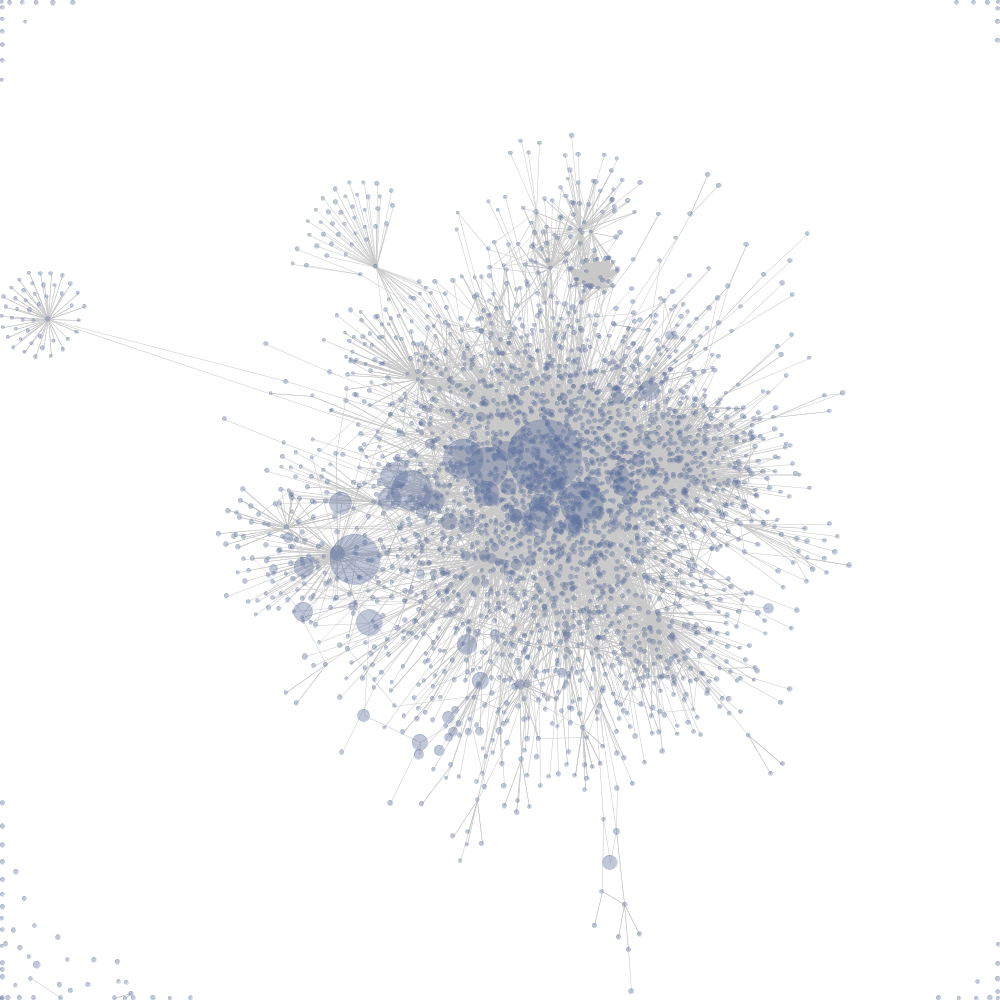
\includegraphics[width=0.85\textwidth]{fdgd_example.png}}
\caption[]{Primjer grafa dobivenog silom usmjerenim crtanjem grafova.\footnotemark}
\label{img:fdgd_example}
\end{figure}
\footnotetext{Izvor: \url{https://en.wikipedia.org/wiki/Force-directed_graph_drawing}}

\section{Grupiranje dokumenata}
Jedna od često korištenih metoda u kontekstu analize i pretraživanja teksta jest grupiranje dokumenata (engl. \textit{document clustering}). Cilj grupiranja jest izdvojiti dokumente neke zbirke u grupe tako da su dokumenti u jednoj grupi na neki način međusobno slični. Primjer jedne grupe dokumenata bili bi dokumenti o nogometu, košarci i odbojci budući da se sva tri dokumenta tiču sportskih aktivnosti. Kako bi se dokumenti mogli svrstati u grupe, potrebno je iskoristiti neki od algoritama za grupiranje. Jedan takav algoritam jest grupiranje \textit{k}-srednjih vrijednosti (engl. \textit{k-means clustering}) \cite{Steinbach2000ACO}.

\subsection{Grupiranje \textit{k}-srednjih vrijednosti}
\label{k_means_clustering}
Grupiranje \textit{k}-srednjih vrijednosti je metoda koja spada u nenadzirano učenje (engl. \textit{unsupervised learning}) te se koristi kada podaci nisu označeni — u kontekstu grupiranja dokumenata to bi značilo da za dokumente nisu unaprijed poznate grupe kojima ti dokumenti pripadaju. Cilj algoritma grupiranja \textit{k}-srednjih vrijednosti jest napraviti upravo to: odvojiti postojeće podatke u \textit{k} grupa (odnosno pronaći iste), po čemu je algoritam i dobio naziv. Algoritam iterativno svakoj točki dodjeljuje grupu ovisno o sličnostima u odnosu na sve ostale točke (u kontekstu grupiranja dokumenata, ta sličnost je upravo mjera sličnosti dokumenata).
Ulaz u algoritam jesu podaci (engl. \textit{dataset}) te parametar \textit{k}.
Na početku se slučajnim mehanizmom odabere \textit{k} grupa nakon čega slijedi ponavljanje sljedeća dva koraka:

\begin{figure}
\centering
\def\svgwidth{\columnwidth}
\input{images/clustering.pdf_tex}
\caption[]{Primjer grupiranja podataka koristeći algoritam \textit{k}-srednjih vrijednosti\footnotemark}
\label{img:clustering}
\end{figure}
\footnotetext{Izvor: \url{http://www.cs.sfu.ca/~ggbaker/data-science/content/ml-other.html}}

\begin{enumerate}
\item \textbf{Dodjela grupa podacima.} U svakom koraku, za svaki podatak odredi se kvadratna euklidska udaljenost do najbliže grupe (tj. njezinog centroida). Formalno, potrebno je pronaći grupu $c_{i}$ takvu da vrijedi:
\begin{equation}
{\displaystyle {\underset{{c_i}\,\in\,C}{\operatorname {arg\,min}}}\,\,dist({c_i},\,x)^2}
\end{equation}
gdje je $dist(c_i, x)$ već spomenuta euklidska udaljenost točke $x$ do centroida $c_i$.
\item \textbf{Ažuriranje centroida.} Za svaku od grupa, radi se ažuriranje centroida na način da se izračuna aritmetička sredina svih točaka koje su dodijeljene dotičnoj grupi.
\begin{equation}
{\displaystyle {c_i}}=\frac{1}{|S_i|} \sum_{x_i\in\,S_i}^{} x_i
\end{equation}
\end{enumerate}
Algoritam dakle iterira kroz opisane korake dok nijedna točka ne promijeni grupu u kojoj se nalazi, odnosno dok ne bude ispunjen neki od uvjeta konvergencije (npr. dosezanje maksimalnog broja iteracija). Demonstracija algoritma prikazana je na slici
\ref{img:clustering_alg}.

\begin{figure}
\makebox[\textwidth]{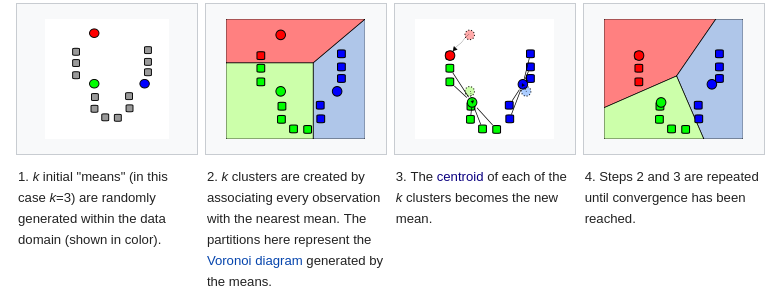
\includegraphics[width=\textwidth]{clustering_alg.png}}
\caption[]{Demonstracija algoritma grupiranja \textit{k}-srednjih vrijednosti\footnotemark}
\label{img:clustering_alg}
\end{figure}
\footnotetext{Izvor: \url{https://en.wikipedia.org/wiki/K-means_clustering}}

\chapter{Programska implementacija}
\label{chap:impl}
Programska implementacija ovog završnog rada napisana je u programskom jeziku Java koji je zbog svoje objektne metodologije, nativne podrške apstraktnih kolekcija podataka te postojane podrške raznih vanjskih biblioteka idealan za implementaciju problema iz domene analize i pretraživanja teksta.
Korištene biblioteke su \textit{Apache PDFBox} za parsiranje PDF dokumenata, \textit{Apache Commons Math} za proračun \textit{k}-srednjih vrijednosti, \textit{Apache Digest Utils} za izračun MD5 sažetka (engl. \textit{hash}) vrijednosti te \textit{Jung} biblioteke za proračun te vizualizaciju grafova. \par
Kao što je već ranije spomenuto, pročitani dokumenti reprezentirani su vektorima obzirom da je to jedan od  najjednostavnijih i najefikasnijih način prikaza dokumenata. Naime, u memoriji se na taj način ne trebaju eksplicitno spremati riječi za svaki dokument već se mogu spremiti samo brojke koje govore koliko je dotična riječ relevantna za dokument. Kako se u sklopu ovog rada koristi TF-IDF reprezentacija dokumenata, to znači da se za svaki dokument treba izračunati njegova TF-IDF (vektorska) reprezentacija. Prije samog izračuna komponenata TF-IDF vektora, potrebno je pročitati PDF dokumente smještene na disku. Pošto su PDF dokumenti zapravo binarne datoteke, po svojoj strukturi nisu trivijalno parsabilni, što znači da ih nije moguće pročitati odnosno dekodirati na jednostavan način kao što je to moguće s primjerice tekstualnim datotekama. Zbog toga se za njihovo čitanje, odnosno parsiranje koristi vanjska biblioteka Apache PDFBox koja iz zadanog PDF dokumenta vadi Unicode znakove koje može pročitati te ih vrati kao rezultat. Tako dobiveni tekst dodatno se obrađuje pri čemu se uklanjaju bilo kakvi interpunkcijski znakovi, dijakritici, brojke, odnosno svi znakovi koji nisu mala ili velika slova engleske abecede.\footnote{Uklanjanje svih znakova koji nisu slova engleske abecede obavlja se jer je programska implementacija predviđena za rad s dokumentima na engleskom jeziku} Ovakav postupak nužan je kako bi se što više smanjio utjecaj nebitnih znakova na točnost uspoređivanja dokumenata.
Jednom kada je tekst isfiltriran, nad njim se provodi daljnja predobrada koja: 1) uklanja iz teksta stop-riječi te 2) vrši stemanje nad dobivenim riječima dokumenata. Obje metode opisane su u potpoglavlju
\ref{subchap:docmodel_docview}. Nakon završene predobrade teksta, stvaraju se vokabular, vektori (za reprezentaciju dokumenata) te nekoliko dodatnih pomoćnih struktura podataka. Nakon ovog koraka vrši se još i izračun sličnosti dokumenata kako bi jednom izračunati podaci bili spremljeni za ponovno korištenje bez da se moraju svaki puta iznova računati.

\section{Čitanje i obrada riječi}
Programsko rješenje ovog završnog rada nudi korisniku interaktivan način pretraživanja postojeće zbirke dokumenata postavljanjem upita kroz grafičko korisničko sučelje. Naime, nakon odabrane putanje do zbirke dokumenata, korisnik postavlja upit te program pretražuje zbirku dokumenata i korisniku prikazuje dokumente sortirane po relevantnosti korisničkom upitu.
Korisnički se upit obrađuje kao što je već ranije spomenuto u poglavlju \ref{docmodel}: zanemaruju se svi znakovi koji nisu slova engleske abecede, uklanjaju se stop riječi, provodi se stemanje te se nakon toga korisnički unos obrađuje -- za svaku riječ provodi se metoda kosinisne sličnosti odnosno BM25 te se od korisničkog unosa izgradi vektor koji taj unos predstavlja u \textit{n}-dimenzijskom koordinatnom sustavu, gdje \textit{n} predstavlja veličinu (broj riječi) vokabulara. Nakon izračuna sličnosti s dokumentima zbirke, program korisniku prikazuje popis svih relevantnih dokumenata, zajedno s odgovarajućim koeficijentima sličnosti.

Za obradu korisničkog upita (odnosno bilo kakvog unosa od strane korisnika, kao što će biti pokazano u iduća dva potpoglavlja) koristi se razred \textit{InputProcessor} iz paketa \textit{hr.fer.zemris.zavrsni.input}. Ovaj razred koristi se kad god treba pročitati tekst zadan od strane korisnika: bilo to kroz korisnički upit, bilo kroz učitavanje dokumenata s diska. Naime, on sadrži popis zaustavnih riječi te reference na primjerke razreda koji implementiraju sučelje \textit{DocumentReader} (kojemu se delegira posao samog čitanja riječi) i \textit{Stemmer} (kojemu se delegira posao stemanja riječi). Razred \textit{Stemmer} predstavlja implementaciju Porterovog algoritma stemanja (engl. \textit{Porter stemming algorithm}) koja je u Javi javno dostupna na Internetskoj stranici samog algoritma.
Pozivatelj (glavni program) na početku kroz statičku metodu razreda postavlja objekt tipa \textit{DocumentReader} koji "zna" kako odraditi čitanje. Razred \textit{InputProcessor} će na početku pozvati metodu \textit{readDocument} objekta \textit{DocumentReader} koji će pročitati sve riječi iz odgovarajućeg izvora riječi. Nakon toga \textit{InputProcessor} koristi \textit{Stemmer} kako bi svim riječima uklonio sufikse te ih sveo na kanonski oblik. Ovako obrađene riječi \textit{InputProcessor} vraća pozivatelju.
\begin{figure}
\makebox[\textwidth]{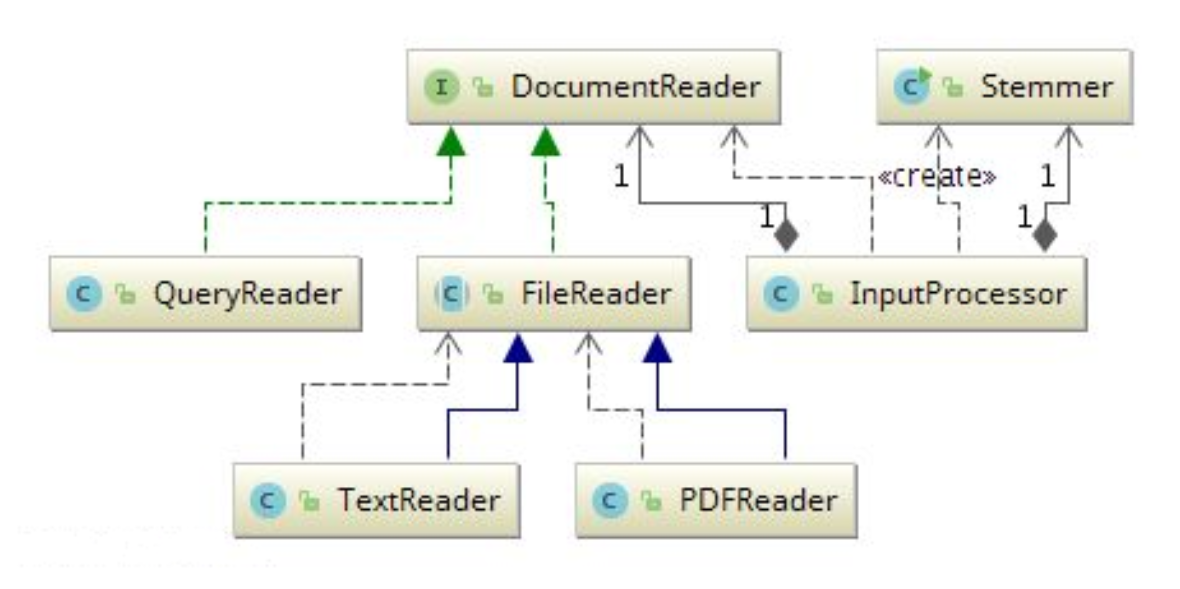
\includegraphics[width=0.85\textwidth]{diagram.png}}
\caption[Dijagram razreda zaduženih za čitanje riječi]{Dijagram razreda zaduženih za čitanje riječi (paket \textit{hr.fer.zemris.zavrsni.input})}
\label{img:diagram}
\end{figure}

\subsection{Obrada korisničkog upita}
Za obradu korisničkog upita zadužen je razred \textit{QueryReader} koji implementira sučelje \textit{DocumentReader} koje predstavlja apstakciju najviše razine za objekte koji obavljaju akciju čitanja. Kada korisnik unese upit u znakovno polje (engl. \textit{text field}), primjerak razreda \textit{QueryReader} sprema zadani unos u privatnu člansku varijablu. Pozivatelj (glavni program) tada postavlja taj primjerak kao \textit{DocumentReader} razreda \textit{InputProcessor} koji tada koristi objekt kako bi dohvatio upit korisnika. Dohvaćeni tekst se nakon toga obrađuje (uklanjanje zaustavnih riječi, steming) te je spreman za daljnju obradu (vektorizacija i sama usporedba s dokumentima).
\begin{figure}
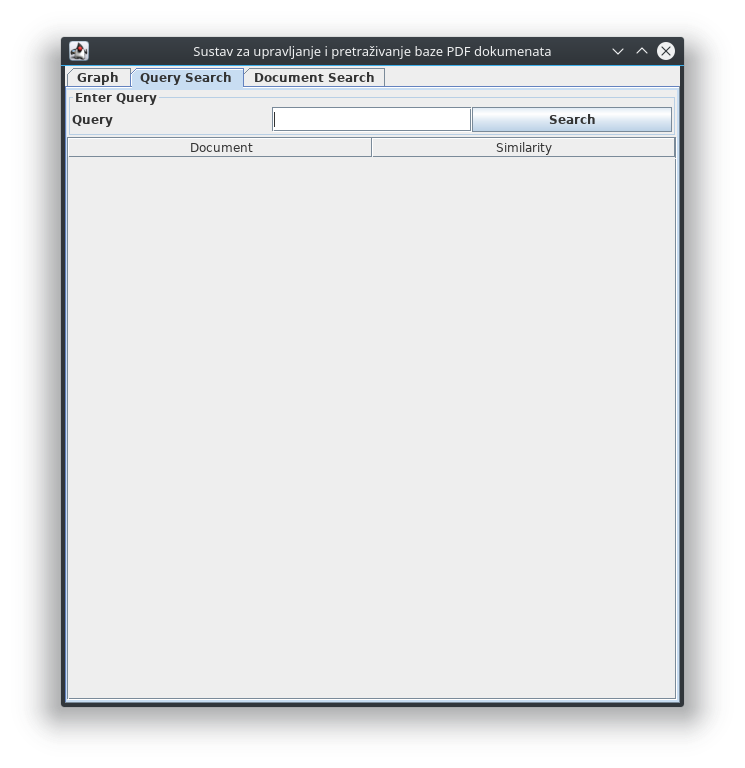
\includegraphics[width=\textwidth]{query_search.png}
\caption{Prikaz dijela programa za unos korisničkog upita}
\label{img:query_search}
\end{figure}

\begin{figure}
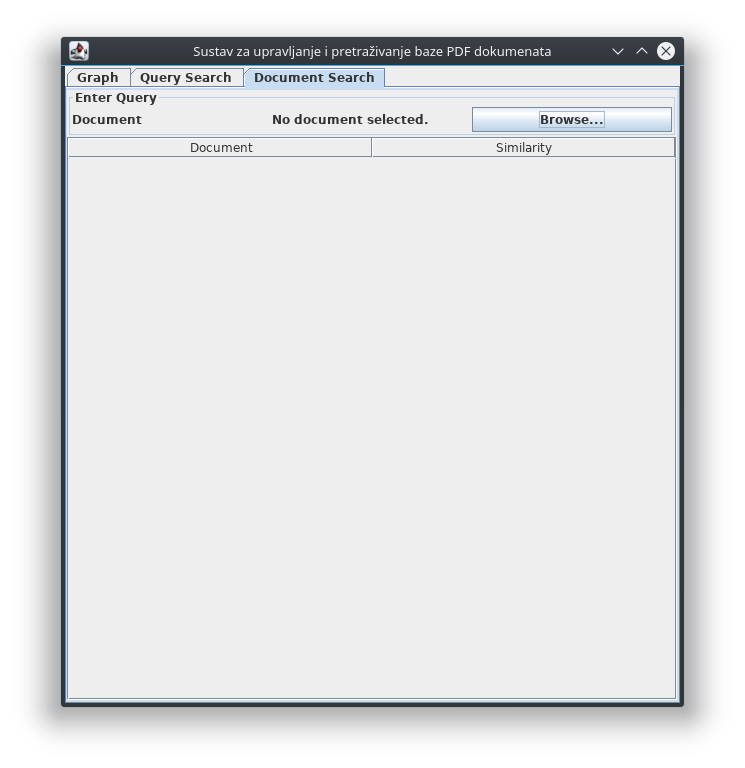
\includegraphics[width=\textwidth]{document_search.png}
\caption{Prikaz dijela programa za odabir proizvoljnog dokumenta}
\label{img:doc_search}
\end{figure}

\subsection{Obrada dokumenata}
Osim pretraživanja zbirke dokumenata prema korisničkom upitu, program nudi mogućnost pronalaska sličnih dokumenata proizvoljno odabranom dokumentu koji se ne nalazi u zbirci. Nakon pokretanja programa i odabira putanje do zbirke dokumenata, korisnik može odabrati proizvoljan dokument s diska kako bi pronašao njemu slične dokumente iz zbirke. Za učitavanje dokumenata s diska (kao i za obradu korisničkog upita), koristi se razred \textit{InputProcessor} koji ne koristi više \textit{QueryReader} kao što to radi prilikom obrade korisničkog upita, već koristi primjerke razreda izvedenih iz apstraktnog razreda \textit{FileReader} — \textit{TextReader} te \textit{PDFReader}. \textit{TextReader} ostvaruje funkcionalnost čitanja riječi iz obične tekstualne datoteke (nastavak \textit{.txt}). Ovaj razred ne koristi se u finalnoj verziji programske implementacije, no bio je vrlo značajan za potrebe testiranja u implementacijskoj fazi izrade programske potpore. Za čitanje PDF dokumenata koristi se \textit{PDFReader} koji pak posao parsiranja samih PDF dokumenata delegira vanjskoj biblioteci \textit{Apache PDFBox}. Tako dohvaćeni tekst se, kao i kod obrade korisničkog upita, nakon toga obrađuje te je spreman za daljnju obradu.

\section{Međusobna usporedba dokumenata}
Nakon što pozivatelj dobije kolekciju riječi od razreda \textit{InputProcessor} (bilo dobivenih iz korisničkog upita ili pročitanih iz dokumenata), stvara njihovu TF-IDF vektorsku reprezentaciju koju modelira razred \textit{Vector} iz paketa \textit{hr.fer.zemris.zavrsni.model}. Tako stvoreni vektor potom se preda javnom konstruktoru razreda \textit{Document} iz istog paketa koji modelira virtualni dokument. \textit{Virtualni} u ovom kontekstu znači da primjerak tog razreda ne predstavlja doslovno dokument koji se nalazi na disku korisnika, već enkapsulira izgrađeni vektor te omogućuje pristup ostalim razredima kroz prikladno definirano sučelje. S druge strane, razred \textit{Document} može predstavljati dokument s diska, kao što je to slučaj s dokumentima iz zbirke. Razred \textit{Document} jest dakle apstrakcija koja predstavlja kolekciju riječi, bez obzira na to odakle dolazi — bilo iz korisničkog upita, bilo iz dokumenta s diska. Ovakvo strukturirano rješenje ima jednu vrlo elegantnu posljedicu: svaka usporedba dokumenta, bez obzira na njegov izvor nastanka u programskom se kodu ostvaruje samo na jednom mjestu. Drugim riječima, nije potrebno raditi razliku između usporedbe različitih "tipova" dokumenata već se svaka usporedba svodi na jednu.

\section{Funkcije rangiranja}
Kao što je već spomenuto u poglavlju \ref{docmodel}, metode istražene u sklopu ovog rada su metoda kosinusne sličnosti te metoda BM25.
Nad objema metodama napravljen je niz ispitivanja: kroz korisničke upite, ali i s proizvoljnim dokumentima. BM25, često smatran \textit{state-of-the-art} tehnikom rangiranja dokumenata se zapravo, kao što je već aludirano u poglavlju \ref{docmodel}, koristi primarno za rangiranje dokumenata. Naime, BM25 po svojoj definiciji ne definira apsolutnu već relativnu mjeru sličnosti; naime, ako se neki dokument usporedi sa samim sobom, rezultat neće nužno biti jednak 1, kao što je to slučaj kod kosinusne metode sličnosti. To posljedično stvara problem jer nije moguće ustanoviti koliko je neki dokument (apsolutno) sličan nekom drugom dokumentu.

Ovom problemu moglo bi se doskočiti normaliziranjem mjere sličnosti na način da se mjera sličnosti između dokumenata $d_1$ i $d_2$ umjesto na klasičan način — \text{similarity}($d_1, d_2$) — računa tako da se dobiveni rezultat podijeli mjerom sličnosti dokumenta $d_1$ (ili $d_2$) sa samim sobom, odnosno
\begin{equation}
\frac{\text{similarity}(d_i, d_j)}{\text{similarity}(d_j, d_j)}.
\label{eq:docsim}
\end{equation}
Na ovaj način, za svaki par dokumenata dobila bi se vrijednost u intervalu [0, 1] što odgovara intervalu kosinusne metode te je poželjno svojstvo u svrhe rangiranja, odnosno pronalaska sličnih dokumenata. \par
No ipak, korištenje ovakve tehnike zaobilazi izvornu svrhu metode Okapi BM25, a to je relativno rangiranje dokumenata po sličnosti. Kako u samoj implementaciji ne bi bilo nedefiniranog, odnosno neočekivanog ponašanja u postupku proračuna sličnosti dokumenata, za potrebe ovog rada odabrana je metode kosinusne sličnosti, koja se bez obzira na svoju naizgled bazičnu strukturu, pokazala vrlo uspješnom ne samo u svrhe pronalaska međusobne sličnosti dokumenata, već i u slučaju apsolutnog rangiranja dokumenata, što je ključan faktor za ispravnu vizualizaciju dokumenata, o čemu će više riječi biti u sljedećem potpoglavlju.

Implementacijski, metode kosinusne sličnosti te BM25, predstavljene su razredima \textit{CosineSimilarity} te \textit{OkapiBM25}. Ovi razredi izvedeni su iz apstraktnog razreda \textit{RankingFunction} koji se, zajedno s konkretnim implementacijama, nalazi u paketu \textit{hr.fer.zemris.zavrsni.ranking}. Kao što je to spomenuto u prethodnom potpoglavlju, sve usporedbe bilo kakvih tipova dokumenata u programskom se kodu događaju na jednom mjestu, odnosno, kroz jedno sučelje. Naime, razred \textit{RankingFunction} sadrži javnu metodu \textit{sim (Document, Document)} koja prima dva generička dokumenta. Konkretne implementacije tog razreda implementiraju svaka svoj način usporedbe dokumenata, u skladu s njihovim definicijama, čime se uklanja potreba za dupliciranjem koda.

\section{Vizualizacija dokumenata}
\label{sec:docdisplay}
Metode definirane u poglavlju \ref{chap:docsin2d} (silom usmjereno crtanje grafova te grupiranje \textit{k}-srednjih vrijednosti) mogu se iskoristiti upravo za prikaz i grupiranje dokumenata, odnosno njihovih međusobnih sličnosti u 2D koordinatnom sustavu. Prije početka ijednog od algoritama, svi dokumenti i pripadajući im vektori moraju biti učitani, odnosno inicijalizirani. Nadalje, za svaki par dokumenata $d_{i}$ i $d_{j}$, $i \neq j$, izračuna se njihova sličnost (koristeći neku od metoda prikazanih u potpoglavlju \ref{subchap:similarity}) te se čvorovi (dokumenti) i bridovi (sličnosti) predaju algoritmu koji odsimulira postupak opisan u potpoglavlju \ref{subchap:forcedir}. Nakon što je algoritam završio sa simulacijom, postupak završava te se prikazuje nacrtani graf.
\begin{figure}
\centering
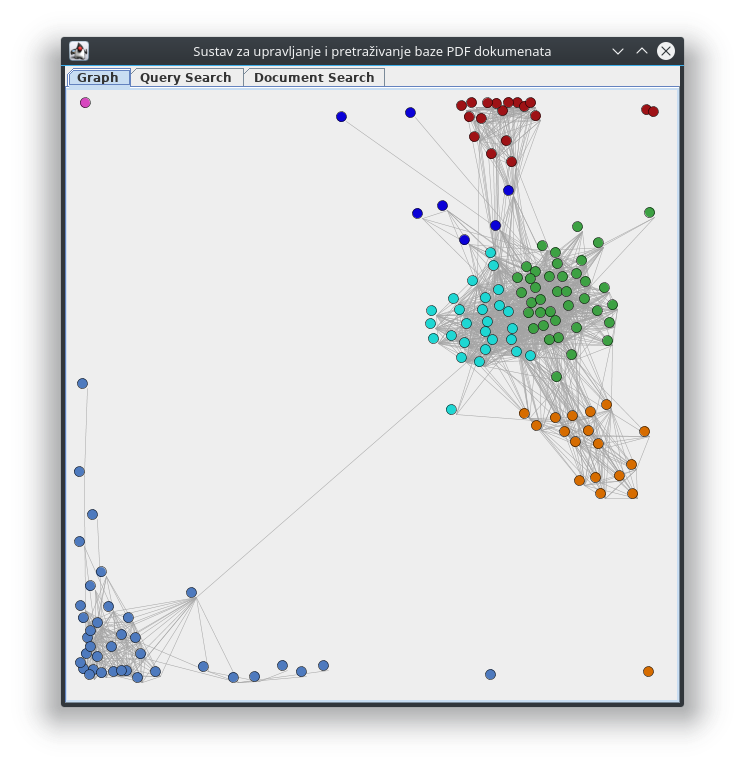
\includegraphics[width=0.85\textwidth]{graph_program.png}
\caption{Prikaz dijela programa za prikaz dokumenta zbirke}
\label{img:graph_program}
\end{figure}
Nad tako nacrtanim grafom dalje se može primijeniti algoritam grupiranja \textit{k}-srednjih vrijednosti koji prvo procjenjuje hiperparametar \textit{k} (o kojem će više riječi biti u potpoglavlju \ref{kmeans_optimization}) te nakon toga provodi postupak grupiranja dokumenata. Nakon što se oba algoritma izvrše, dobiveni rezultat jest upravo prikaz dokumenata u 2D koordinatnom sustavu s naznačenim grupama koje predstavljaju aproksimaciju (broja) grupa dokumenata iz zbirke. \par
Primjena algoritma \textit{k}-srednjih vrijednosti na grupiranje dokumenata jest sljedeća: grupirati dokumente u \textit{k} grupa na način da se svakom dokumentu — točki u 2D prostoru koja ga predstavlja — dodijeli grupa do čijeg je centra ta točka najbliža. Algoritam započinje tako da slučajnim mehanizmom odabere \textit{k} grupa te dodijeli dokumente u najbliže im grupe. Nakon inicijalne dodjele u grupe, računa se novih \textit{k} grupa te se postupak iterativno ponavlja do konvergencije. Nakon završenog postupka, svaki će se dokument nalaziti u najbližoj mu grupi, zajedno s ostalim dokumentima koji su mu najsličniji.
Nažalost, grupiranje dokumenta u ovome kontekstu nije izravno moguće zbog toga što algoritam apriorno (lat. \textit{a priori}) nema informaciju o broju grupa dokumenata iz zbirke. Razlog tome jest sama priroda problema koji se rješava, a to je da su na početku nepoznate grupe dokumenata (kao i njihov broj), odnosno jedini podaci dostupni programu su sami dokumenti. No ipak, broj grupa zbirke, \textit{k}, ipak se može procijeniti određenim heuristikama kao što će biti pokazano u potpoglavlju \ref{kmeans_optimization}.

\section{Optimizacija izvođenja programa}
Kako bi program bio što responzivniji na upite korisnika, nakon što se po prvom pokretanju programa izvrši čitav postupak inicijalizacije dokumenata (predobrada dokumenata, stvaranje vokabulara, računanje sličnosti dokumenata itd.), dobiveni se podaci spremaju u pričuvnu (engl. \textit{cache}) memoriju, odnosno bivaju serijalizirani (engl. \textit{serialization}) na disk. Svrha ovog postupka jest jednom dobivene i izračunate relevantne podatke zbirke dokumenata spremiti u perzistentnu memoriju računala kako bi se po svakom sljedećem pokretanju programa, umjesto ponovnog prikupljanja i izračuna svih relevantnih podataka, isti mogli efikasnije isčitati iz zapisane datoteke te deserijalizirati u odgovarajuće strukture podataka čime se uvelike dobiva na brzini izvođenja programa. U tablici
\ref{table:serialization} vidljivo je da se korištenjem serijalizacije postiže prosječno ubrzanje od čak 58 puta prilikom svakog (ne-inicijalnog) pokretanja programa.

\begin{table}
\begin{center}
\begin{tabular}{|c|c|c|}
\hline
Br. dokumenata & Ponovno čitanje (sek) & Deserijalizacija (sek) \\
\hline
7 & 63.94 & 0.76 \\
157 & 670.81 & 21.05 \\
\hline
\end{tabular}
\end{center}
\caption{Usporedba trajanja ponovnog čitanja dokumenata i deserijalizacije}
\label{table:serialization}
\end{table}

\section{Provjera integriteta zbirke dokumenata}
Kako bi program bio u mogućnosti autonomno detektirati promjene nad zbirkom dokumenata (primjerice, ako je novi dokument dodan, ako je neki dokument uklonjen itd.), koristi se tehnika provjere kontrolne sume (engl. \textit{checksum}) dokumenata. Naime, nakon što korisnik odabere direktorij na disku koji predstavlja zbirku dokumenata, nad njim se provede rekurzivan postupak izračuna MD5 sažetka svakog od dokumenata u tom direktoriju. Dobiveni sažetci se tada usporede s postojećim sažetcima koji su spremljene u posebnoj pričuvnoj datoteci. Ukoliko se vrijednosti poklapaju, program zaključuje kako nad zbirkom nije bilo nikakvih promjena od zadnjeg pokretanja te učitava prethodno serijalizirane podatke o zbirci dokumenata i uskoro postaje spreman za korištenje. Ako je međutim uočena razlika između postojećih i izračunatih sažetaka (ili ako oni prethodno uopće ne postoje), očito je da je zbirka promijenjena (ili prethodno niti nije bila serijalizirana) te se nanovo računaju svi relevantni podaci koji se potom serijaliziraju u odgovarajuću pričuvnu datoteku kako bi bili dostupni prilikom sljedećeg pokretanja.

\begin{code}[caption={Isječak programskog koda za provjeru ispravnosti zbirke},captionpos=b]
private static boolean isDatasetCorrect(Path dataset) {
    String md5 = new MD5Visitor(dataset).getMd5();
    String md5Real;

    if (new File(md5Filename).exists()) {
        md5Real = IOUtils.readFromTextFile(md5Filename);

    } else {
        IOUtils.writeToTextFile(md5Filename, md5);
        return false;
    }

    if (new File(datasetInfoFilename).exists()) {
        if (md5.equals(md5Real)) {
            return true;

        } else {
            IOUtils.writeToTextFile(md5Filename, md5);
            return false;
        }

    } else {
        return false;
    }
}
\end{code}

\section{Optimizacija hiperparametra \textit{k} algoritma \textit{k}-srednjih vrijednosti}
\label{kmeans_optimization}
Kao što je već spomenuto u potpoglavlju \ref{k_means_clustering}, određivanje hiperparametra \textit{k} nije izravno moguće jer algoritmu grupiranja \textit{k}-srednjih vrijednosti (štoviše, niti cijelome programu) nije dostupna informacija o broju grupa. Ovaj podatak inherentno je nepoznat cijelome programu jer što prije početka izvođenja programa nije poznato koliko se grupa nalazi u zbirci dokumenata. Štoviše, jedan od ciljeva implementacije ovog rada jest i automatsko grupiranje dokumenata koje pak ne mora nužno biti egzaktno, u smislu da točno odredi koji dokumenti spadaju u koju grupu dokumenata. Naime, ako bi takvo grupiranje bilo relevantno, tada nastaje problem definicije grupe dokumenata. Budući da, je sličnost dokumenata po definiciji kontinuirana vrijednost, nije moguće odrediti "granicu" koja će odrediti kada neki dokument prestaje pripadati jednoj, a počinje pripadati drugoj grupi. Zbog ovog razloga, a i zbog inherentnog nepoznavanja broja grupa od strane korisnika na početku izvođenja programa, parametar \textit{k} nije moguće odrediti sa sigurnošću.
\begin{figure}
\makebox[\textwidth]{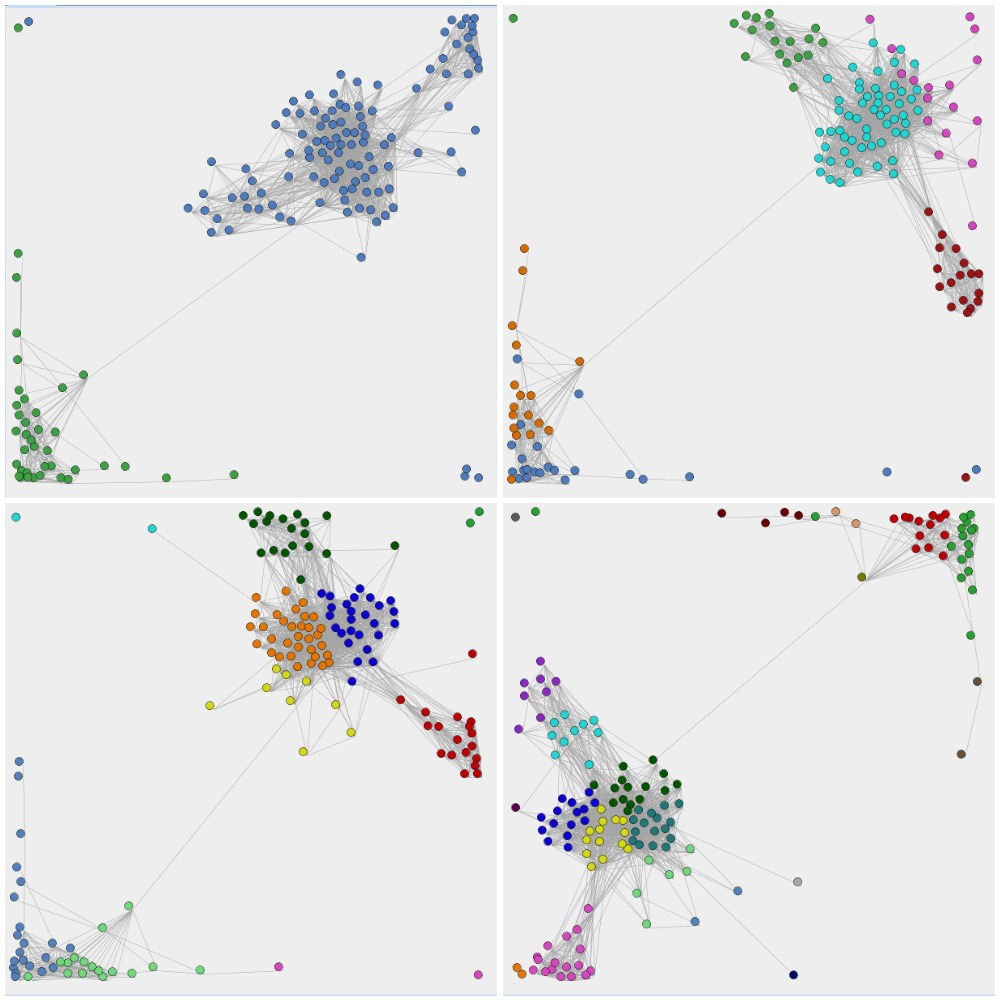
\includegraphics[width=\textwidth]{join.jpg}}
\caption[Dijagram razreda zaduženih za čitanje riječi]{Rezultat algoritma grupiranja \textit{k}-srednjih vrijednosti za proizvoljno odabrane vrijednosti parametra \textit{k}: \textit{k=2}, \textit{k=6}, \textit{k=10} te \textit{k=20}}
\label{img:graph_kmeans}
\end{figure}
\begin{figure}[h]
\centering
\def\svgwidth{\columnwidth}
\input{images/elbow.pdf_tex}
\caption[]{Ovisnost vrijednosti pogreške o parametru \textit{k}\footnotemark}
\label{img:elbow}
\end{figure}
\footnotetext{Izvor: https://averisera.uk/machine-learning-clustering.html}

Kako bi se riješio problem određivanja parametra \textit{k}, moguće je iskoristiti određene heuristike koje procjenjuju parametar na temelju empirijskih podataka. Jedna relativno dobra heuristika za optimiranje parametra \textit{k} jest metoda koljena.

\subsection{Metoda koljena}
Metoda koljena (engl. \textit{elbow method}) je jedna od metoda za određivanje broja grupa. Ideja metode je jednostavna: algoritam \textit{k}-srednjih vrijednosti iterativno se izvede za vrijednosti \textit{k} u nekom rasponu (npr. [1, 10]) te se u svakoj iteraciji izračuna suma srednjih kvadratnih pogrešaka (engl. \textit{residual sum of squares, RSS}) udaljenosti svake od točaka do centroida dodijeljene joj grupe. Nakon izvršenog postupka, bit će izračunate sume kvadratnih pogrešaka za svaku od iteracija koje su se izvršile, odnosno za svaku vrijednost parametra \textit{k} iz prethodno zadanog raspona. Nakon izvršenog postupka, za svaku od vrijednosti parametra \textit{k} nacrta se pripadajuća suma kvadratnih pogrešaka te se promotri u kojoj točki (tj. za koji \textit{k}) se nalazi "koljeno", u smislu najvećeg pada vrijednosti sume pogreške. Jedan takav primjer prikazan je na slici \ref{img:elbow} na kojoj se jasno vidi veliko smanjenje pogreške između \textit{k=1} i \textit{k=2} što znači da će se kao vrijednost parametra \textit{k} uzeti vrijednost 2 zbog toga što je upravo za tu vrijednost pronađen najveći pad pogreške, što ukazuje na to da je algoritam pronašao optimalan broj grupa. Čitatelj bi se mogao zapitati zbog čega se kao broj grupa onda ne uzme neka veća vrijednost, primjerice onu za koju je pogreška najmanja (nula). No odgovor na ovo je jednostavan: kada bi suma pogrešaka bila nula, to bi značilo da bi broj grupa bio upravo jednak broju dokumenata. No ovo nema smisla, pošto se u kontekstu ovog problema želi grupirati više dokumenata u grupe. Zaključak je dakle da treba odabrati takvu vrijednost parametra \textit{k} za kojeg je pad pogreške najveći. Ovakav odabir skoro uvijek bit će optimalan.
Metoda koljena bila bi idealna za optimizaciju parametra \textit{k} kada bi postojala jednostavna metoda određivanja samog "koljena". No ovdje nastaje problem programskog određivanja točke najvećeg pada pogreške. Tom problemu moguće je doskočiti drugim heuristikama koje bi bile zadužene za pronalazak koljena, no u tom slučaju je rješenje problema postalo novi problem kojeg treba riješiti te razina apstrakcije time značajno raste. Ovakav pokušaj nema previše smisla za automatizirano računanja, stoga ova metoda nažalost nije dovoljno dobra u kontekstu ovog rada. U sljedećem potpoglavlju bit će pokazana još jedna heuristika koja se može iskoristiti za problem određivanja parametra \textit{k}.

\subsection{Metoda korijena}
Metoda korijena jest jednostavna heuristika koja pokušava procijeniti parametar \textit{k} na sljedeći način:
\begin{equation}
{k}={\mathbf {\sqrt{|\textit{D}| \over 2}}},
\end{equation}
gdje je $D$ zbirka dokumenata. Ovakva heuristika ne dovodi nužno do optimalnog rješenja (tj. do egzaktnog broja grupa), no služi kao relativno dobra aproksimacija, što je u ovome kontekstu često puta sasvim dovoljno. Primjerice, za zbirku dokumenata u kojoj na početku postoje dvije jasno odvojene grupe, npr. engleski nogomet i srednjevjekovno mačevanje, zanimljivo je promotriti kako parametar \textit{k} ovisi o broju dokumenata u pojedinoj grupi.

\begin{table}
\begin{center}
\begin{tabular}{|c|c|c|}
\hline
Grupa I. (br. dok.) & Grupa II. (br. dok.) & \textit{k} \\
\hline
3 & 4 & 1.87 \\
5 & 5 & 2.24 \\
11 & 17 & 3.74 \\
42 & 53 & 6.87 \\
\hline
\end{tabular}
\end{center}
\caption{Ovisnost parametra \textit{k} o broju dokumenata pojedine grupe}
\label{table:kmeans}
\end{table}

U tablici \ref{table:kmeans}, zanimljivo je uočiti kako porast broja dokumenata zbirke dovodi do pogrešne aproksimacije broja grupa. Naime, očito je (prilikom konstrukcije gornjeg izraza) empirijski ustanovljeno kako svaka od grupa u prosjeku nema prevelik broj dokumenata, zbog čega aproksimacija za velik broj dokumenata nažalost daje (vrlo) pogrešne rezultate — u ovom konkretnom primjeru, za približno 10-ak dokumenata po grupi, pogreška aproksimacije parametra \textit{k} doseže čak 100\%! Ovaj podatak govori o problematici heuristika: često puta daju dovoljno dobru aproksimaciju, no ponekad mogu i poprilično pogriješiti.
No ipak, zaključak isprobavanja različitih metoda u svrhu ovog rada jest da je metoda korijena donijela najbolju aproksimaciju broja grupa zbirke dokumenata te se iz tog razloga koristi u konačnoj verziji implementacije programske potpore.

\chapter{Diskusija rezultata}
\label{chap:results}
Za potrebe testiranja implementacije te kasnije analize dobivenih rezultata, u sklopu ovog rada koristila se unaprijed pripremljena zbirka dokumenata opisana u tablici \ref{table:datasetinfo}. Korištena zbirka sadrži 148 članaka i dokumenata iz sljedećih raznovrsnih područja: arhitektura, astronomija, biologija, filozofija, kemija te računarska znanost. Ovakva struktura zbirke dokumenata za potrebe prototipiranja i testiranja programske implementacije odabrana je kako bi bila vidljiva:
\begin{itemize}
\item[$\bullet$] sličnost dokumenata srodnih područja (npr. kemija i biologija),
\item[$\bullet$] razlika dokumenata različitih područja (npr. kemija i arhitektura).
\end{itemize}

\begin{table}
\begin{center}
\begin{tabular}{|c|c|c|}
\hline
Grupa & Broj dokumenata \\
\hline
Arhitektura & 17 \\
Astronomija & 25 \\
Biologija & 24 \\
Filozofija & 19 \\
Kemija & 20 \\
Računarska znanost & 43 \\
\hline
$\sum$ & 148 \\
\hline
\end{tabular}
\end{center}
\caption{Prikaz broja dokumenata po grupama}
\label{table:datasetinfo}
\end{table}

Uvid u prethodno opisane informacije (a posebice vizualizacija spomenutih sličnosti odnosno razlika dokumenata) mogao bi dati potencijalno vrlo zanimljive rezultate. Primjerice, za očekivati je da će srodni dokumenti međusobno imati veću mjeru sličnosti nego dokumenti nepovezanih područja. Tako bi recimo bilo sasvim prirodno vidjeti dokumente iz područja kemija i biologije kako su vizualno međusobno blizu, dok bi dokumenti iz kemije i arhitekture bili relativno razdvojeni. Rezultati međusobnih sličnosti dokumenata već spomenute zbirke prikazani su slikom \ref{img:turing} koja je direktan rezultat pokretanja programa nakon učitavanja zbirke.

\begin{figure}
\makebox[\textwidth]{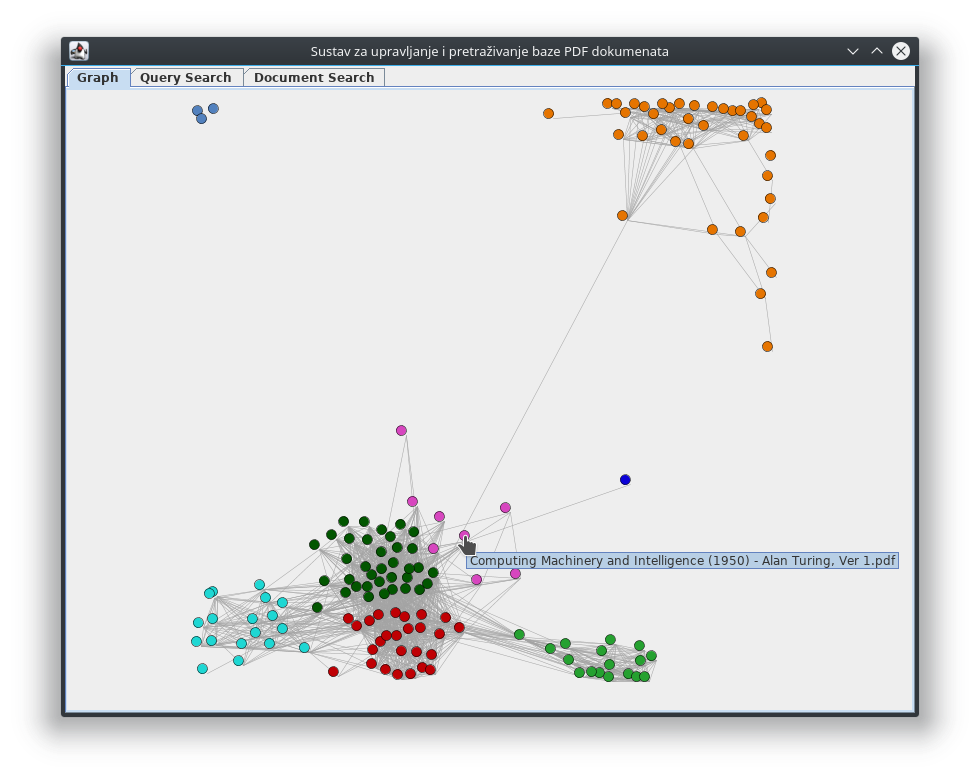
\includegraphics[width=0.85\textwidth]{turing.png}}
\caption{Grafički prikaz sličnosti dokumenata korištene zbirke}
\label{img:turing}
\end{figure}

Na slici se može vidjeti 6 jasno istaknutih grupa: tirkizna, tamno-zelena, crvena, ružičasta, svijetlo-zelena te narančasta. Tirkizna boja prikazuje dokumente iz područja biologije, crvena i svijetlo-zelena dokumente astronomije i arhitekture (tim redoslijedom) a narančasta prikazuje dokumente iz područja računarske znanosti. Tamno-zelena i ružičasta grupa nisu navedene iz razloga što ne prikazuju isključivo jednu grupu dokumenata; tamno-zelena boja prikazuje dokumente iz područja biologije (gornja polovica) i područja filozofije (donja polovica), dok ružičasta boja također prikazuje dokumente iz biologije i filozofije, no prikazuje i jedan posebno zanimljiv dokument čiji se naziv vidi u info-oblačiću (engl. \textit{tooltip}) na slici. Naime, znanstveni rad \textit{Computing Machinery and Intelligence} kojega je 1950. godine objavio Alan Turing \cite{turing2009computing}, jedan od pionira računarstva i umjetne inteligencije, prikazan je veoma blizu dokumenata iz područja filozofije. Ovakav raspored na prvi pogled može se doimati čudnim; bilo bi prirodno pretpostaviti da će rad o umjetnoj inteligenciji biti dodijeljen grupi dokumenata o računarskoj znanosti. No budući da se rad velikim dijelom bavi pitanjima poput: "Mogu li računala razmišljati?" te budući da se rad bavi raznim misaonim pokusima, postaje očito da je rad zapravo vrlo filozofske naravi te da ima posve smisla što je postavljen upravo u kontekst filozofskih dokumenata. Osim spomenutih, postoji još nekoliko grupa (svijetlo-plava i tamno-plava) koje sadrže vrlo mali broj dokumenata. Dokumenti prikazani u tim grupama nisu semantički pripali u nijednu drugu grupu te su dobili vlasitite grupe. Očito je kako rezultat vizualizacije dokumenata neće uvijek biti optimalan, pa čak niti posve smislen.

Još jedna zanimljivost koju valja uočiti sa slike \ref{img:turing} jest ta da su dokumenti iz područja računarske znanosti (narančasta boja) neobično udaljeni od svih ostalih grupa dokumenata; interpretacija se ostavlja čitatelju za vježbu.

\section{Prikaz rezultata korisničkog upita}

Osim grafičkog prikaza sličnosti dokumenata, valja promotriti i rezultate dobivene postavljanjem upita, odnosno učitavanjem proizvoljnih dokumenata koji će potom biti uspoređeni s dokumentima iz zbirke. Slika \ref{img:astronomy_query} prikazuje pretraživanje zbirke uz upit "Stars are made of hot plasma"\footnote{Pošto su dokumenti zbirke svi na engleskom jeziku, pretraživanje ima smisla samo koristeći upite na engleskom jeziku.}. Iz dobivenih rezultata, jasno je kako uneseni upit najveću sličnost ima upravo s dokumentima iz područja astronomije (10.7\% sličnosti s najsličnijim dokumentom).

Jedan potencijalan nedostatak modela vreće riječi korištenog za prikaz dokumenata u jest taj da se njegovim korištenjem u potpunosti zanemaruje poredak riječi te se ne koristi nikakva sofisticiranija analiza poput npr. semantičke. Problem nastaje kada se primjerice zada upit od nekoliko riječi koje predstavljaju neki izraz (npr. akronim). Sustav baziran na modelu vreće riječi, na postavljeni upit neće gledati kao na to što zapravo jest (semantički smisleni izraz) već naprosto na neporedanu kolekciju riječi. Dakle, u kontekstu vreće riječi, postaje posve svejedno hoće li korisnik napisati upit "Plavo nebo i zelene doline" ili "Doline nebo i zelene plave" -- što naravno nema smisla. Ovakav pristup potencijalno bi mogao donijeti pogrešne rezultate ovisno o korisnikovoj namjeri prilikom unošenja upita, odnosno o izrazu po kojem pokušava pretraživati.

\begin{figure}
\centering
{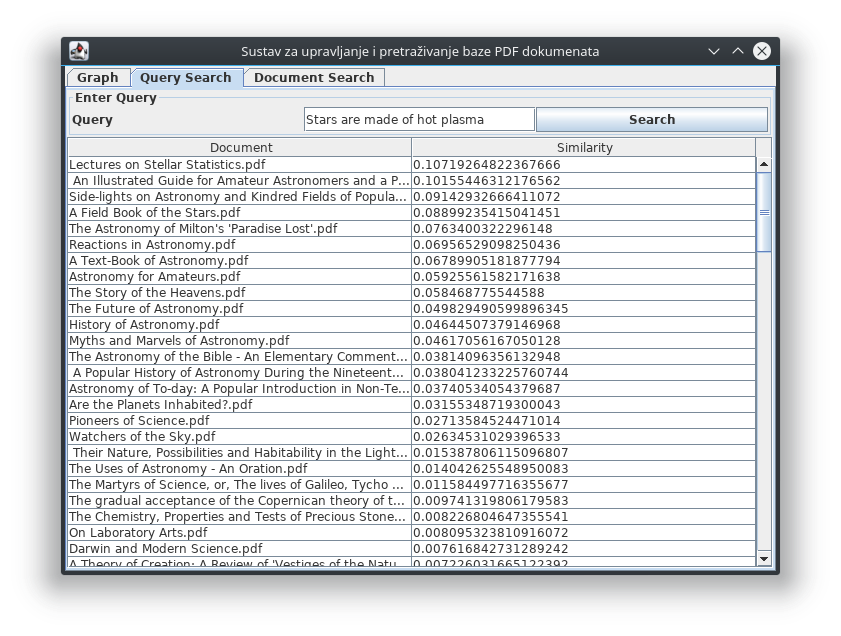
\includegraphics[width=0.9\textwidth]{astronomy_query.png}}
\caption{Prikaz rezultata nad unesenim korisničkim upitom}
\label{img:astronomy_query}
\end{figure}

\section{Prikaz rezultata učitanog dokumenta}

Još preostaje pogledati rezultate dobivene usporedbom proizvoljno učitanog dokumenta s postojećom zbirkom -- kao primjer je ovdje korišten rad \textit{Distributed Representations of Sentences and Documents} \cite{le2014distributed}. Iz rezultata sa slike \ref{img:document_query}, vide se slično očekivani rezultati kao i u prethodnom primjeru: znanstveni rad koji se bavi prikazom rečenica i dokumenata najsličniji je dokumentima iz područja računarske znanosti, što se i vidi po 2.48\% sličnosti s najsličnijim dokumentom.

\begin{figure}
\centering
{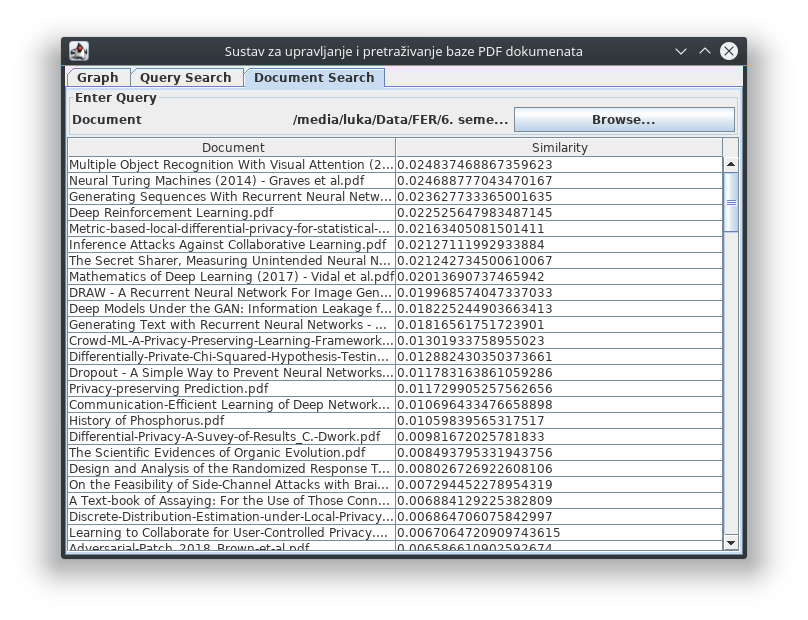
\includegraphics[width=0.9\textwidth]{document_query.png}}
\caption{Prikaz rezultata nad učitanim dokumentom}
\label{img:document_query}
\end{figure}

\chapter{Zaključak}
U ovome radu iznesena je ideja usporedbe dokumenata po sličnosti u svrhe pronalaska semantički sličnih dokumenata te rangiranja dokumenata prema korisničkom upitu (odnosno proizvoljno učitanom dokumentu). Napravljena je implementacija koja korisniku omogućava upravljanje i pretraživanje lokalne baze PDF dokumenata.

Kao metoda uspoređivanja dokumenata korištena je metoda kosinusne sličnosti. Za vizualizaciju dokumenata korištena je metoda silom usmjerenog crtanja grafova. Za grupiranje dokumenata korištena metoda \textit{k}-srednjih vrijednosti.

Pripremljeni dokumenti iz sadržajno sličnih grupa generalno su grafički bili prikazani relativno blizu, dok nepovezani dokumenti nisu; ovakvo je ponašanje očekivano te je shodno tome programska implementacija dala zadovoljavaće rezultate.

Daljni smjer i razvoj mogao bi biti u smjeru unaprijeđenja modela prikaza dokumenata; naime, model vreće riječi u nekim je situacijama vrlo naivan pristup problematici analize teksta u usporedbi sa sofisticiranijim modelima koji uzimaju u obzir poredak riječi, njihovu međusobnu sličnost (pronalazak sinonima) i sl.

Analiza i pretraživanje dokumenata po sličnosti svakim je danom sveobuhvatnije područje u svijetu tehnologije te ima brojne primjene pa je stoga unaprijeđenje metoda analize teksta u svrhu preciznijeg i učinkovitijeg pretraživanja teksta neophodno za daljnji razvoj područja, pa i znanosti i tehnologije uopće.

\bibliography{literatura}
\bibliographystyle{fer}

\begin{sazetak}
Pretraživanje i uspoređivanje dokumenata vrlo je rašireno u današnjem svijetu. Sve više raznih područja iziskuju nekakvu vrstu pretraživanja odnosno dohvata informacija iz teksta. Da bi se to moglo ostvariti, potrebno je poznavati metodologiju usporedbe dokumenata po sličnosti. U okviru ovog rada istažene su neke od takvih metoda te je napravljena implementacija koja korisniku nudi mogućnost upravljanje lokalnom bazom PDF dokumenata. Bazu je moguće pretraživati koristeći tekstualni upit ili proizvoljni dokument. Dokumenti baze također se mogu se grafički prikazati pri čemu će biti vidljiva njihova međusobna sličnost. Programska implementacija ostvarena je u programskom jeziku Java.

\kljucnerijeci{Sličnost dokumenata, TF-IDF, Vizualizacija dokumenata, Grupiranje \textit{k}-srednjih vrijednosti, Java}
\end{sazetak}

% TODO: Navedite naslov na engleskom jeziku.
\engtitle{PDF Document Management and Search System}
\begin{abstract}
Searching and comparing documents is very widespread in today's world. Many different areas require some kind of information retrieval. In order to accomplish that, it is necessary to be familiar with the methodology of document comparison. This thesis explores some of these methods which are then used for an implementation which enables the user to manage a local database of PDF documents. The database can be searched by a textual query or an arbitrary document. The documents' similarities can also be shown graphically. The implementation was written in the Java programming language.

\keywords{Document similarity, TF-IDF, Document visualization, K-means clustering, Java}
\end{abstract}

\end{document}